\documentclass[output=paper,colorlinks,citecolor=brown,
% hidelinks,
% showindex
]{langscibook}

\author{Francisco Antonio Monta\~no \affiliation{Lehman College, City University of New York (CUNY)}} 
\title{The long and short of prothesis in early French word-initial /sC/ clusters}

%It is very important to upload our abstract in this portion of the document. This will allow search engines like google scholar to locate your research to be showcased to the world. Just replace the Latin text contained within the curly brackets below with your text. Make sure to keep the curly open and end brackets!
\abstract{This paper argues for a more abstract account of the intersecting Old French (OF) processes of prothesis and 12th-13th century coda /s/ deletion, the latter accompanied by compensatory lengthening (\textit{feste} [fɛs.tə] > [fɛ:.tə]).  In close chronological proximity, the prothetic vowel of etymological word-initial /sC/ becomes fixed, suggesting prothesis' shift from phrase- to word-level.  But once /s/ cannot occupy coda position, simple prothesis no longer yields a harmonic output. Though /s/ deletes in prothesis clusters (\textit{espouse} [es.pu.zə] > [e.pu.zə]), compensatory lengthening does not accompany deletion as occurs word-internally. Given this disparity, I claim an abstract analysis where /sC.../ remains underlying. Arguing against a moraic analysis of /s/ deletion \citep{Gess1998} in light of the reflexes of prothesis clusters, I link both phenomena in diachrony with the Split Margin Approach \citep{baertschdavis2003} and root node preservation.  Coda /s/ deletion in prothesis clusters thus represents a distinct evolution of prothesis whereby the only licit segment in this position, a vowel, overtakes the position of unharmonic initial /s/. The new input-output mapping of /sC/ $\rightarrow$ [eC] makes late OF prothesis a case of non-surface-apparent opacity \citep{McCarthy1999}. My analysis captures the synchronic intersection of the opaque prothesis phenomenon and /s/ deletion within a unified account compatible with the anticipated life cycle of phonological processes \citep{Bermúdez-Otero2015} and suggestive evidence from /sC/-initial stems' behavior in morphological concatenation.} %Change Latin filler with your own abstract.

\IfFileExists{../localcommands.tex}{%hack to check whether this is being compiled as part of a collection or standalone
   % add all extra packages you need to load to this file

\usepackage{tabularx,multicol,multirow}
\usepackage{url}
\urlstyle{same}

\usepackage{listings}
\lstset{basicstyle=\ttfamily,tabsize=2,breaklines=true}

\usepackage{langsci-basic}
\usepackage{langsci-optional}
\usepackage{langsci-lgr}
\usepackage{langsci-gb4e}
%    \let\eachwordone=\it % Ch 14, 18

\usepackage{jambox}
\usepackage{subfigure}
\usepackage{tablefootnote}
\usepackage[nameinlink, noabbrev]{cleveref}
\crefname{enumi}{example}{examples}

\usepackage{bbding}
%\usepackage{linguex}
\usepackage{stmaryrd}

\usepackage{tipa}
\let\ipa\textipa
\usepackage{vowel}
\newcommand{\BlankCell}{}
\usepackage{ot-tableau}

\usepackage{forest}
\useforestlibrary{linguistics}
\usepackage[noeepic]{qtree}
\usepackage{pstricks, pst-xkey, pst-jtree}
\usepackage{tikz-qtree}
\usepackage{tikz-qtree-compat}
\usepackage{tree-dvips}

\usepackage{lastpage}
\usepackage{hyperref}
\usepackage{xltxtra}

\usepackage{ragged2e}
%\usepackage{subcaption}
\usepackage{floatrow}
\usepackage{float}

\usepackage[normalem]{ulem} % Pour les textes barrés
\usepackage{ifthen} 

\usepackage{todonotes}

   \newcommand*{\orcid}{}

\makeatletter
\let\theauthor\@author
\makeatother

\papernote{\scriptsize\normalfont
    \theauthor.
    \titleTemp. 
    To appear in: 
    Chad Howe and Pilar Chamorro and Timothy Gupton and Margaret Renwick.
    Theory, Data, and Practice: Selected papers from the 49th Linguistic Symposium on Romance Language
    Berlin: Language Science Press. [preliminary page numbering]
}

% Workaround for subscripts with capital letters
\newcommand{\capsub}[1]{\ensuremath{_\text{#1}}}

% Chapter 10: Table-like presentation within example environment
% classical latin > {*}late latin > old french  earlier > later   gloss
\newcommand{\montanoboxi}[7]{\parbox{2cm}{#1} > {#2}\parbox{2cm}{#3} > \parbox{1.5cm}{\textit{#4}} \parbox{1.2cm}{#5}\ > \parbox{1.2cm}{#6} \parbox{1.5cm}{#7}}
% {*}latin > earlier OF [ipa] > early OF   gloss
\newcommand{\montanoboxii}[6]{{#1}\parbox{1.9cm}{\textit{#2}} > \parbox{1.3cm}{\textit{#3}} \parbox{2cm}{#4} \parbox{2cm}{#5} \parbox{1.9cm}{#6}}

% Chapter 5
\newcommand{\redc}[1]{\textcolor{red}{#1}}
\newcommand{\bluec}[1]{\textcolor{blue}{#1}}
\newcommand{\ajout}[1]{\textcolor{blue}{#1}}
\newcommand{\ajoutplus}[1]{\textcolor{cyan}{#1}}

\newcommand{\hachure}[9]{
% Parametres :
% Coordonnees bas gauche (2 parametres) : (#1,#2)
% Coordonnees haut droit (2 parametres) : (#3,#4)
% Orientation : #5
%   1 : diagonale de pente 1
%  -1 : diagonale de pente -1
%   0 : horizontal
%   2 : vertical
% Nombre de pas horizontaux : #6
% Epaisseur du trait : #7
% Couleur : #8 (ex. green)
% Atténuation couleur : #9 (ex. 30)
\pgfmathsetmacro{\N}{#6-1}
\pgfmathsetmacro{\A}{#1}
\pgfmathsetmacro{\B}{#2}
\pgfmathsetmacro{\C}{#3}
\pgfmathsetmacro{\D}{#4}
\pgfmathsetmacro{\I}{(#3-#1)/#6}
\pgfmathsetmacro{\J}{(#4-#2)/#6}
\ifthenelse{\equal{#5}{1}}{
  \foreach \n in {0,...,\N}
    \foreach \m in {0,...,\N}
      {
        \pgfmathsetmacro{\X}{\A + ((0 + \n) * \I)}
        \pgfmathsetmacro{\Y}{\B + ((0 + \m) * \J)}
        \pgfmathsetmacro{\U}{\A + ((1 + \n) * \I)}
        \pgfmathsetmacro{\V}{\B + ((1 + \m) * \J)}
        \draw[#8!#9,#7] (\X, \Y)--(\U, \V);
      } 
  }{}
\ifthenelse{\equal{#5}{-1}}{
  \foreach \n in {0,...,\N}
    \foreach \m in {0,...,\N}
      {
        \pgfmathsetmacro{\X}{\A + ((1 + \n) * \I)}
        \pgfmathsetmacro{\Y}{\B + ((0 + \m) * \J)}
        \pgfmathsetmacro{\U}{\A + ((0 + \n) * \I)}
        \pgfmathsetmacro{\V}{\B + ((1 + \m) * \J)}
        \draw[#8!#9,#7] (\X, \Y)--(\U, \V);
      } 
  }{}
\ifthenelse{\equal{#5}{0}}{
  \foreach \n in {0,...,\N}
    \foreach \m in {0,...,\N}
      {
        \pgfmathsetmacro{\X}{\A + ((0 + \n) * \I)}
        \pgfmathsetmacro{\Y}{\B + ((0 + \m) * \J)}
        \pgfmathsetmacro{\U}{\A + ((1 + \n) * \I)}
        \pgfmathsetmacro{\V}{\B + ((0 + \m) * \J)}
        \draw[#8!#9,#7] (\X, \Y)--(\U, \V);
      } 
  }{}
\ifthenelse{\equal{#5}{2}}{
  \foreach \n in {0,...,\N}
    \foreach \m in {0,...,\N}
      {
        \pgfmathsetmacro{\X}{\A + ((0 + \n) * \I)}
        \pgfmathsetmacro{\Y}{\B + ((0 + \m) * \J)}
        \pgfmathsetmacro{\U}{\A + ((0 + \n) * \I)}
        \pgfmathsetmacro{\V}{\B + ((1 + \m) * \J)}
        \draw[#8!#9,#7] (\X, \Y)--(\U, \V);
      } 
  }{}
}

%Définition d'un pattern de type hachure
% \usetikzlibrary{patterns}
% \makeatletter
% \tikzset{hatch distance/.store in=\hatchdistance,hatch distance=5pt,hatch thickness/.store in=\hatchthickness,hatch thickness=5pt}

% \pgfdeclarepatternformonly[\hatchdistance,\hatchthickness]{north east hatch}% name
%     {\pgfqpoint{-\hatchthickness}{-\hatchthickness}}% below left
%     {\pgfqpoint{\hatchdistance+\hatchthickness}{\hatchdistance+\hatchthickness}}% above right
%     {\pgfpoint{\hatchdistance}{\hatchdistance}}%
%     {
%         \pgfsetcolor{\tikz@pattern@color}
%         \pgfsetlinewidth{\hatchthickness}
%         \pgfpathmoveto{\pgfqpoint{-\hatchthickness}{-\hatchthickness}}       
%         \pgfpathlineto{\pgfqpoint{\hatchdistance+\hatchthickness}{\hatchdistance+\hatchthickness}}
%         \pgfusepath{stroke}
%     }
% \pgfdeclarepatternformonly[\hatchdistance,\hatchthickness]{north west hatch}% name
%     {\pgfqpoint{-\hatchthickness}{-\hatchthickness}}% below left
%     {\pgfqpoint{\hatchdistance+\hatchthickness}{\hatchdistance+\hatchthickness}}% above right
%     {\pgfpoint{\hatchdistance}{\hatchdistance}}%
%     {
%         \pgfsetcolor{\tikz@pattern@color}
%         \pgfsetlinewidth{\hatchthickness}
%         \pgfpathmoveto{\pgfqpoint{\hatchdistance+\hatchthickness}{-\hatchthickness}}
%         \pgfpathlineto{\pgfqpoint{-\hatchthickness}{\hatchdistance+\hatchthickness}}
%         \pgfusepath{stroke}
%     }
% \makeatother
%~~~~~~~~~~~~~~~~~~~~~~~~~~~~~~~~~~~~~


% Chapter 7
\newcommand\pef[1]{(\ref{#1})}

\newcommand{\subscript}[1]{\textsubscript}

   %% hyphenation points for line breaks
%% Normally, automatic hyphenation in LaTeX is very good
%% If a word is mis-hyphenated, add it to this file
%%
%% add information to TeX file before \begin{document} with:
%% %% hyphenation points for line breaks
%% Normally, automatic hyphenation in LaTeX is very good
%% If a word is mis-hyphenated, add it to this file
%%
%% add information to TeX file before \begin{document} with:
%% %% hyphenation points for line breaks
%% Normally, automatic hyphenation in LaTeX is very good
%% If a word is mis-hyphenated, add it to this file
%%
%% add information to TeX file before \begin{document} with:
%% \include{localhyphenation}
\hyphenation{
anaph-o-ra
Dor-drecht
%FFI2016-76045-P-AEI/-MINEICO/-FEDE
}

\hyphenation{
anaph-o-ra
Dor-drecht
%FFI2016-76045-P-AEI/-MINEICO/-FEDE
}

\hyphenation{
anaph-o-ra
Dor-drecht
%FFI2016-76045-P-AEI/-MINEICO/-FEDE
}

    \bibliography{localbibliography}
    \togglepaper[23]
}{}

\begin{document}
\maketitle
\section{Introduction}
	In this paper, I argue for a new analysis of the interaction between Old French (OF) prothesis (\textit{spede} [spe.ðə] > \textit{espee} [es.pe.ə] > [e.pe] 'sword') and coda /s/ deletion (\textit{feste} /fɛstə/ $\rightarrow$ [fɛ:.tə] 'feast').  Prothesis inserts a non-underlying vowel or consonant as a repair on a non-harmonic phonological sequence in word- or stem-initial position \citep{Sampson2010}.  Vowel prothesis is particularly well represented in Romance, be it in standard or regional varieties, or diachronically:

\ea \label{ex:montano:1}
	Examples of prothesis in Romance
\ea Italian diachrony (15th century Florentine):\\\textit{escritta} cf. standard \textit{scritta} 'written'; \textit{ispendere} cf. standard \textit{spendere} 'spend-\textsc{inf}' \citep{Sampson2003}
\ex Latin (Lat.) loanwords from Greek:\\\textit{πτερισ} > \textit{ipteridus} 'fern'; \textit{ξιφιον} > \textit{exsifion} 'gladiolus' \citep{Passino2013}
\ex OF:\\(Lat. \textit{sponsare} >) \textit{esposer} (> Fr. \textit{épouser}) 'wed-\textsc{inf}' \citep{Pope1952}; (Lat. \textit{spat(h)a} >) \textit{espethe} (> Fr. \textit{épée}) 'sword' \citep{Sampson2010}
\ex Portuguese diachrony:\\(Lat. \textit{scutu} >) \textit{escudo} 'shield'; (Lat. \textit{strictu} >) \textit{estreito} 'narrow' \citep{Lief2006}
\ex Spanish loanwords from English:\\'stress' > \textit{estrés}, 'scanner' > \textit{escáner} \citep{BernáSicilia2011}
\z\z

\noindent The insertion of the initial vocalic segment allows the heterosyllabic realization of an otherwise illicit word-initial consonant cluster; in the Romance examples in (\ref{ex:montano:1}) above, the offending cluster is sibilant-obstruent (/sC/), and in the Late Latin examples, obstruent-obstruent.  Essentially, a consonant sequence banned as a complex onset instead surfaces as coda + onset following the inserted vowel (/C\textsubscript{1}C\textsubscript{2)|}.../ $\rightarrow$ [VC\textsubscript{1}.C\textsubscript{2}...]), preserving both segments and thereby escaping alternative anti-faith repairs such as deletion (/C\textsubscript{1}C\textsubscript{2}.../ $\rightarrow$ [C\textsubscript{2}...], e.g. Greek \textit{πτισανη} > Lat. \textit{tisana} 'herbal tea' \citep{Passino2013}) or feature modification (e.g. Portuguese diachrony: /plato/ > [prato] 'plate', etc., cf. \citet[116--118]{Lief2006}).  The word-initial cluster, despite its markedness, surfaces faithfully but heterosyllabically.

In OF (11th-13th centuries), lexical items descending from etyma with word-initial /sC/ (i.e. prothesis clusters) exhibit a prothetic vowel ([esC...]), as in (\ref{ex:montano:2}): 

\ea\label{ex:montano:2} Prothesis of word-initial sibilant-obstruent clusters from Late Latin to OF (data from 	\citealt{Pope1952, Rohlfs1970, Sampson2010, Montaño2017})\\
    \hspace{0.5cm} \montanoboxi{Class. Lat.}{}{Late Lat.}{OF}{(earlier}{later)}{Gloss}
    \ea \montanoboxi{[spatula]}{ }{[is.pa.tu.la]}{espalle}{[ɛs.p..]}{[e.p...]}{`shoulder'}
    \ex \montanoboxi{[skrip.tum]}{*}{[is.krip.tu]}{escrit}{[ɛs.k...]}{[e.k...]}{`written'}
    \ex \montanoboxi{[sk(h)o.lam]}{*}{[is.ko.la]}{escole}{[ɛs.k...] }{[e.k...]}{`school'}
    \ex \montanoboxi{[spon.sai]}{ }{[is.po.sɛ]}{espuse(s)}{[ɛs.p...]}{[e.p...]}{`wives'}
\z\z

In later OF, prothesis seemingly intersected with the well-documented process of coda /s/ deletion \citep{Pope1952, Gess1998, Gess1999, baertschdavis2003, Sampson2010}.  Data in (\ref{ex:montano:3}) show word-medial /s/ deletes pre-consonantally, that is, when it would syllabify as a coda:
\ea \label{ex:montano:3}
  \ea\label{ex:montano:3a} 11th-12th c. OF: Loss of medial coda /s/ – allophone [z] \citep{Pope1952} \\
  \hspace{0.5cm} \montanoboxii{\phantom{*}}{\textnormal{Latin}}{\textnormal{Earlier}}{\textnormal{OF}}{Early OF}{Gloss}
    \ea\label{ex:montano:3aa} \montanoboxii{\phantom{*}}{insula \\(> *isola)}{isle}{[iz.lə]}{[i:.lə]}{`island'}
    \ex\label{ex:montano:3ab} \montanoboxii{\phantom{*}}{hispidum}{hisde}{[iz.də]}{[i:.də]}{`horror'}
    \ex\label{ex:montano:3ac} \montanoboxii{*}{blastemare}{blasmer}{[blaz.mer]}{[bla:.mer]}{`accuse-\textsc{inf}'}
    \ex\label{ex:montano:3ad} \montanoboxii{\phantom{*}}{misculare}{mesler}{[mez.ler]}{[mɛ:.ler]}{`mix-\textsc{inf}'}
	\z
  \ex\label{ex:montano:3b} Later OF (13th c.): Loss of medial coda /s/ – allophone [s] \citep{Pope1952} \\
  \hspace{0.5cm} \montanoboxii{\phantom{*}}{\textnormal{Latin}}{\textnormal{Earlier}}{\textnormal{OF}}{Early OF}{Gloss}
    \ea\label{ex:montano:3be} \montanoboxii{\phantom{*}}{festa}{feste}{[fɛs.tə]}{[fɛ:.tə]}{`feast'}
	\ex\label{ex:montano:3bf} \montanoboxii{\phantom{*}}{noster}{nostre}{[nɔs.trə]}{[nɔ:.trə]}{`our.SG'}
	\ex\label{ex:montano:3bg} \montanoboxii{*}{sponsare}{esposer}{[es.po.zer]}{[e.pu.zer]}{`wed-\textsc{inf}'}
	\ex\label{ex:montano:3bh} \montanoboxii{*}{frisca}{fresche}{[fres.tʃə]}{[frɛ:.ʃə]}{`fresh-F.SG'}
	\ex\label{ex:montano:3bi} \montanoboxii{*}{(e)skutarju}{escu(d)ier}{[es.ky.(ð)i.er]}{[e.ky.jer]}{squire}
	\ex\label{ex:montano:3bj} \montanoboxii{*}{excappare}{eschaper}{[es.tʃa.per]}{[e.ʃa.per]}{`escape-\textsc{inf}'}	      
	\z
\z\z
 


\noindent 
The diachronic French literature \citep{Pope1952, Nyrop1914, Bourciez1955, Gess1998, Gess1999} describes coda /s/ deletion as inducing compensatory lengthening on the preceding vowel, with data like \ref{ex:montano:3ac} and \ref{ex:montano:3ad} showing that compensatory lengthening also affected unstressed syllables (cf. \textit{ostel} [ɔ:.'tɛl] 'lodging', \textit{gastel} [ga:.'tɛl] 'cake', \textit{chastel} [tʃa:.'tɛl] 'castle).  Evidence for two stages of coda /s/ deletion, corresponding to its voiced and voiceless allophones, includes poetic rhymes indicating the non-pronunciation of /s/ (e.g. \textit{meïsmes} : \textit{veïmes} \citep{Pope1952}) and the differential transmission of /s/ in Middle English loanwords from OF: e.g. \textbf{hid}eous, bl\textbf{am}e, etc. vs. fe\textbf{ast}, \textbf{esp}ouse, etc. \citep{Pope1952, Gess1999}.

While it is not controversial that word-medial coda /s/ deletion induced vowel lengthening, this account glosses over the critical detail that a once-prothetic vowel purportedly remained short, as \citet{Pope1952} claims in her data (\ref{ex:montano:3bg},\ref{ex:montano:3bi}); I will briefly discuss \ref{ex:montano:3bj} as representing the same in \sectref{sec:montano:2} below).  While both tonic and pretonic syllables may lengthen due to coda /s/ deletion, Pope's data consistently indicate a short vowel in late OF prothesis clusters.  All other diachronic data I have encountered showing /s/ deletion in prothesis clusters (e.g. \citet{Nyrop1914, Bourciez1955}) also show a short prothetic [e] upon /s/ deletion.

A very fair question is if the prothetic vowel might have first lengthened but then shortened due to lack of perceptual salience in an atonic syllable, but I do not believe the evidence supports this claim.  To investigate potential evidence of prothetic vowels having once been long, studying rhymes as in \citet{Gess2001} to identify length contrasts in tonic syllables cannot be used to clarify the same in atonic syllables; different indicators are needed.  An interesting example highlighting long-short vowel pronunciations, though several centuries after late OF, comes from the poetry of 16th century Francien poet Jean-Antoine de Baïf.  Baïf uses his own purportedly phonetic graphical system to elucidate the strong-weak-weak or strong-strong syllabic feet required in his adherence to ancient Greek hexameter (see \citet{Morin1999, Morin2000} for a much more detailed description of his prosodics).  My brief survey of approximately 300--400 verses from the first seven psalms in Baïf's 1573 \textit{Psautier} \citep{Bettens2008} shows pretonic long vowels abound (e.g. \textit{mêlée}, \textit{abîma}, \textit{arêté}, \textit{mâchoire}, \textit{aprêt[e]rai}, \textit{tu lez â pris}, \textit{movêtié [= mauvaistié]}, \textit{lâcheté}), both in graphically-represented vowel length as well as by virtue of occupying the strong position of the foot, while not a single erstwhile prothetic vowel bears such indicators of length (\textit{épine[s]}, \textit{étoit}, \textit{étranjiers}, \textit{ékrivans}, \textit{étreint}, \textit{étourdis}, \textit{étonés}).  This asymmetry is suggestive of a very different reflex in prothetic vowels in contrast with lengthened vowels in atonic syllables.

Further indirect evidence of historical length can be deduced from ulterior vowel quality shifts in non-high long vowels brought to Nouvelle France and still preserved in contemporary Canadian French (CF), a conservative descendant of Francien \citep{Gess2001, Gess2008, Picard2004}.  While one might claim that long vowels in CF examples like \textit{m}[ɛ:]\textit{ler}, \textit{bl}[ɑ:]\textit{mer}, \textit{c}[o:]\textit{té}, \textit{t}[ɛ:]\textit{tu}, \textit{m}[ɛ:]\textit{trise} \citep{Walker1984, Picard2004} may have withstood atonic shortening due to paradigmatic analogical forces (Morin 2000), I find it much harder to say the same for lexemes where the long vowel is unstressed in all related forms, such as \textit{m}[ɑ:]\textit{tin} < \textit{mastin} 'guarddog,' (cf. \textit{m}[a]\textit{tin} 'morning), \textit{ch}[ɑ:]\textit{teau} 'castle'/\textit{ch}[ɑ:]\textit{telain} 'lord,' \textit{ch}[ɑ:]\textit{tier} 'punish,' [o:]\textit{tel} 'lodging', etc.  While examples can be found of certain words not preserving a long vowel reflex from late OF coda /s/ deletion (e.g. \textit{témoin} < \textit{tesmoin} < \textit{testimónium} 'witness', \textit{mélange} 'mixture'), this is far from the rule.  Atonic shortening likely applied only variably across the lexicon.  But if it also affected once-prothetic vowels, why would it have applied categorically only there?  In light of this supporting evidence, I conclude, in agreement with \citet{Pope1952}, that these vowels must have remained short despite the /s/ deleting.

This disparity exposes an oversimplification of how OF prothesis and coda /s/ deletion must have intersected and calls for a more nuanced account of the interplay between the two processes.  In this paper, I present an alternate analysis that supports a more abstract representation of OF prothesis clusters and provides an explanation for their synchronically opaque surface form once coda /s/ deletion had applied.  I claim that the reflexes of OF prothesis clusters, despite the lack of concomitant vowel lengthening, fall out from the same phonological constraints governing coda /s/ deletion.  Before presenting my analysis, several historical details pertaining to French prothesis merit discussion, both to frame the analysis and to define its scope within the lexicon.

\section{History of prothesis in French phonology}\label{sec:montano:2}
In present-day French, vestiges of a once-active prothesis process are clear in the descendants of Latin /sC/-initial words (\textit{école} < \textit{schola} 'school,' \textit{épouse} < \textit{sponsa} 'wife,' etc.).  Despite abundant lexical evidence for historical prothesis, Middle and Renaissance French (15th-16th c.) loanwords from Latin as well as Italian (via Occitan, \citealt{Sampson2003}) appear with or without prothesis as in \textit{(e)scorpion}, \textit{(e)spécial}, \textit{(e)stable}, etc., with mostly the non-prothetic form becoming established in the lexicon \citep{Pope1952, Sampson2003, Montaño2017}.  More recent loanwords likewise do not trigger prothesis in French (e.g. \textit{stress} [stχɛs] < English 'stress', cf. Spanish \textit{estrés} [es.tres]), nor is it attested in popular word formation processes like \textit{verlan}: [stik.mi] < \textit{mystique} [mi.stik] \citep{Sampson2010}.  By Renaissance French, prothesis ceases to apply, leading to initial [sC]'s widespread proliferation in the lexicon; in fact, one brief lexicographic survey finds that [sC] is now one of the more common word-initial cluster types in French \citep{Montaño2017}.
	
Contemporary French [sC]-initial words consist predominantly of loanwords and stand in contradistinction to the "native" lexicon, the focus of this study.  I characterize as "native" those words evolving naturally from /sC/-initial Latin etyma, exhibiting prothesis, and later, OF coda /s/ deletion. In the contemporary language, these words thus exhibit initial /eC.../ (orthographic \textit{éC-}, e.g. \textit{étudiant} 'student', \textit{épouse} 'wife', etc.).  Excluded are learned and semi-learned words like \textit{espérer} 'hope-\textsc{inf}', \textit{espoir} 'hope', \textit{esprit} 'spirit', candidates for OF /s/ deletion but seemingly unaffected via the sociolinguistic force of their ecclesiastical use and connotation \citep{Pope1952}, as well as 15th-16th century French loanwords from Latin and Italian, as their lexical integration dates after late OF, and they thus "miss the boat" for overlapping prothesis and coda /s/ deletion.

OF prothesis of initial /sC/ clusters dates back to Late Latin, when it is evidenced in popular inscriptions \citep{Pope1952, Rohlfs1970, Sampson2003}, and persists into Gallo-Romance (GR).  Evidence of active prothesis abounds in early Medieval Latin scribal texts from the GR geographic zone, as assiduously compiled by \citet{Sampson2010}, including the graphic representation of prothesis (7th c. \textit{istabilis}, 8th c. \textit{estudiant}),  early GR loanwords from Germanic (6th-8th c. Frankish \textit{skum} > \textit{escume} 'foam'; 10th-11th c. Norse \textit{Sten-hūs} > \textit{Étainhus} 'place name'; 11th-13th c. Middle Dutch \textit{stapel} > \textit{estappe} > \textit{étape} 'stage'), and hypercorrections removing non-prothetic etymological vowels before an /sC/ cluster (7th c. \textit{structus} < \textit{i(n)structus}, \textit{strumentum/extromento} < \textit{i(n)strumentum}).  Hypercorrections underscore the probable merger in GR of etymological /VsC/ with /sC/ in many cases, as etymology became obscured.  I would claim this for words like \textit{eschaper} (\ref{ex:montano:3bj}), despite the initial vowel seemingly representing the etymological reflex of the \textit{ex-} prefix.  It is reasonable to presume that GR learners, unaware of the etymological nature of the initial [e] vowel, would deduce that the initial segmental sequence [estʃ...] formed a class underlyingly with the vast number of other [esC]-initial words, positing /stʃaper/ for \textit{eschaper}.  An obvious parallel is found in words like \textit{escharpe} 'pouch', an early borrowing from Germanic *\textit{skerpa} 'basket' \citep{Pope1952}, whose surface phonetic form is indistinguishable synchronically from eschaper.  Examples like this abound in Sampson's (\citeyear{Sampson2010}) findings from 6th-century GR Latin texts such as \textit{spoliarent} (= \textit{expoliarent}), \textit{spectat} (= \textit{exspectat}) and \textit{spiravit} (= \textit{exspiravit}), showing the initial vowel corresponding to etymological \textit{ex-} or \textit{in-} was equated to initial /sC/ even by learned scribes.  The general populace acquiring GR no doubt did the same, and likely more extensively.

Up through OF, prothesis was active in the phrase-level phonology, in stratal terms \citep{Kiparsky2015}, as previous research shows \citep{Pope1952, Rohlfs1970, Sampson2010}.  It applied to /sC/-initial words when not preceded by a vowel-final word, as after vowel-final words /sC/ can split heterosyllabically (/...V\#sCV.../ $\rightarrow$ [...Vs.CV...]).  Early examples from \citet{Pope1952} and \citet{Sampson2010} like \textit{une spede} 'a sword' (9th c. \textit{La Cantilène de Sainte Eulalie}) and \textit{ta/la spuse} 'your/the wife' (early 12th c. \textit{La Vie de Saint Alexis}, ms. L) represent the lack of post-vocalic phrasal prothesis graphically (vs. \textit{out esposede} 'had-3SG wed' [\textit{ibid.}, l. 77]), but examples are scarcer in the 12th century and exist alongside prothetic counterexamples showing pre-vocalic elision (\textit{s'espede} 'his sword' \leftarrow /sa\#spede/ and \textit{l'esposet} 'her=weds' \leftarrow /la\#spo.../ [\textit{ibid.}, ll. 76, 52]).  The variable application of phrasal prothesis points to a process in decline in early OF \citep{Sampson2010}.  By the later 12th century, prothesis applies consistently even after a preceding vowel-final word, as seen in elided forms \textit{s'espee} 'his sword' and \textit{l'estandart} 'the banner' \leftarrow /lə\#standart/ (\textit{Chanson de Roland}, ms. Digby, ll. 346, 3267 \citep{Pope1952}) and its post-vocalic application after non-eliding words (e.g. \textit{tu establiras} 'you establish-\textsc{fut}', \textit{la meie esperance} 'my hope' (mid-12th c. Anglo-Norman Oxford Psalter \citep{Sampson2010}).  The pervasiveness of the prothetic vowel confirms the narrowing of prothesis' domain to the word by the mid-12th century, if not earlier.

In addition to word-level prothesis, later OF features deletion of word-medial coda /s/, as shown in (\ref{ex:montano:3}).  Contemporaneously with coda /s/ deletion, the sibilant in the [es.C...] reflexes of prothesis clusters deletes, fitting neatly with the word-medial ban on coda /s/.  Prothesis seemingly "feeds" – in a diachronic progression rather than in a synchronic generative dimension – coda /s/ deletion by positioning it for syllabification as a coda (/sC.../ $\rightarrow$ [es.C...]).  Presumably, once phrase-level prothesis ceases to yield surface alternations, acquirers of OF from around the mid-12th century onwards would have posited, via lexicon optimization, an underlying form for erstwhile /sC/-initial words including the once-prothetic [e] (/esC.../), thus priming such lexical items for coda /s/ deletion (/esC.../ > [e.C...]).
 
If the above is correct, it is therefore unsurprising to see prothesis words included as examples evidencing OF coda /s/ deletion, as in (\ref{ex:montano:3ab}).  But while the simplicity of the "prothesis-feeds-deletion" analysis is appealing and straightforward, it does not capture all the empirical details.  The most glaring shortcoming, as discussed above, is that compensatory lengthening does not seem to have accompanied /s/ deletion in prothesis clusters, in contradistinction to that attested in word-medial coda /s/ deletion.  The latter mirrors the vowel length or diphthongization that accompanied other OF coda phenomena such as coda nasal deletion, coda /l/ vocalization, and coda /r/ effacement in certain dialects \citep{Gess1998, Gess1999, baertschdavis2003}.  Gess (\textit{ibid.}) offers a compelling account of these coda loss phenomena as due to ever-stricter sonority-based mora-licensing constraints on codas, with compensatory lengthening preserving abandoned moras.
 
But prothesis clusters prove problematic for both a moraic analysis and for the prothesis-feeds-deletion account, leading to analytical contradictions given the short prothetic vowel.  In the moraic account, the otherwise plausible claim that the prothetic vowel had become underlying leaves the short vowel reflex in prothesis clusters unexplained (/esC.../ $\rightarrow$ [e.C...], *[e:.C...]).  Even if the prothetic vowel is treated as non-underlying, it then becomes unclear why /s/ must delete, as it is not in a potential coda position and thus not subject to mora-licensing constraints.  Yet /s/ indeed deletes in this environment as well.  Systemic contradictions such as these call for a more nuanced explanation that captures the diachronic reflexes of /s/ deletion in both prothesis clusters and word-medially, while making the correct predictions regarding the length of the preceding vowel.  I therefore propose a new analysis explaining this disparity, in which I claim that /s/ deletion in prothesis clusters is in fact a phenomenon fundamentally distinct (though interrelated) from the more generalized OF coda /s/ deletion process.

\section{A new analysis of /s/ deletion in word-initial and word-medial /sC/ clusters}
In this section, I detail an analysis that accounts for the differential lengthening effects of OF coda /s/ deletion in both word-medial and prothesis clusters.  This account hinges on Pope's (\citeyear{Pope1952}) claim that the prothetic vowel remained short upon /s/ deletion, which I propose is due to it remaining non-underlying into later OF (i.e. [esC...] remained underlyingly /sC/).  Given that prothesis clusters had ceased to alternate in surface forms around the mid-12th century, this claim is by nature abstract and thus requires justification.  In support of this hypothesis, I consider several reasons why the less abstract underlying /esC.../ representation is problematic as well as evidence supporting underlying /sC.../ in later OF.

The short vowel reflex of prothesis clusters after the loss of /s/ poses the most important piece of evidence against underlying /esC.../.  Though the analysis that OF coda loss phenomena triggered compensatory lengthening \citep{Gess1998, Gess1999} carries traction in word-medial position, the same constraint interaction achieving this should presumably apply to underlying /esC.../, a prediction not borne out empirically.  A mora-preservation analysis predicts a long vowel reflex for /esC.../, e.g. \textit{espuse} $\rightarrow$ *[e:.pu.zə] 'wife', since in a multi-tier phonology both the underlying once-prothetic vowel and the pre-consonantal /s/ would project moras to be preserved in output, as occurs word-medially.  In fact, this prediction likely played out in the \textit{langue d'oc} dialect of Notre-Dame-de-Sanilhac, where the reflex of native prothesis clusters is a diphthong, i.e. bimoraic: cf. [ei.sa.lɔ], [ei.pi.nɔ], [ei.ko.lɔ] < Lat. \textit{scala} 'scale', \textit{spina} 'thorn', \textit{schola} 'school' \citep[135]{Sampson2010}.  This suggests that the prothetic vowel was re-analyzed as underlying and therefore assigned a mora, as was /s/.  On the other hand, OF exhibits a bimoraic reflex in some words where the initial /esC.../ sequence is etymological, as in \textit{estre} 'be-\textsc{inf}' (< *\textit{es're} < Lat. \textit{essere}), which upon /s/ deletion exhibits a long vowel [ɛ:.trə] still retained in some present-day varieties like CF \citep{Walker1984}.  That a bimoraic output is not attested in OF once the /s/ of prothesis clusters deletes supports the claim that the prothetic vowel was not present in the input.

But this claim alone is not even sufficient to formalize the attested evolution of OF prothesis clusters, for if they are indeed underlyingly /sC/, and if /s/ deletion targets /s/ when it will be syllabified as a coda or when mora-bearing, we encounter the next conundrum of why the /s/ must delete at all, if underlyingly it is neither in position to be a coda nor moraic.  To unpack this issue, it is crucial to re-imagine how OF coda /s/ deletion arises from constraint interaction and to re-think precisely which constraints achieve concomitant /s/ deletion and the attested compensatory lengthening.  The OF data in (\ref{ex:montano:3}) and the arguments above already point to the insufficiency of the moraic approach to account for the empirical facts of coda /s/ deletion, since the process occurs in stages depending on the nature of the following onset \citep{Montaño2017}.  Whereas \citet{Pope1952} and \citet{Gess1998, Gess1999} cite surface allophones [z] or [s] as conditioning /s/ deletion in stages (i.e. coda [z] deletes prior to coda [s]), the synchronic reality of /s/ allophony and its consequent pre-consonantal deletion or preservation hinges on the type of onset /s/ precedes.  Moreover, if /s/ deletion were truly the product of mora-licensing constraints, the paradox detailed above follows: underlying initial /esC/ predicts compensatory lengthening upon /s/ deletion, thus yielding empirically incorrect vowel length in output, but underlying /sC/ puts /s/ in non-moraic position, leaving deletion unexplained.  These issues pose serious challenges to a moraic account of /s/ deletion in light of the reflexes of prothesis clusters.

I therefore propose that coda /s/ deletion is more convincingly characterized as a repair on an unharmonious syllable-contact cluster, as characterized in the Split Margin Approach (\textsc{sma}) to the syllable \citep{baertschdavis2003, BaertschDavis2009, GreenBaertsch2014}.  The \textsc{sma} is particularly appropriate for the current analysis, due to its ability to evaluate and make implicational predictions on the relative markedness of both onset and syllable-contact clusters (\textsc{scc}s), as well as its high granularity for referencing all sonority permutations within clusters.  In its representation of the syllable, the \textsc{sma} builds on widely-accepted and well-supported generalizations regarding the relative markedness of high and low sonority segments in the outer (M\textsubscript{1}) and inner (M\textsubscript{2}) margins of the syllable and formalizes a critical structural link between the sonority of consonants on both sides of the syllable peak, as represented below in \figref{fig:montano:SMAsyllable}: 

\begin{figure}
    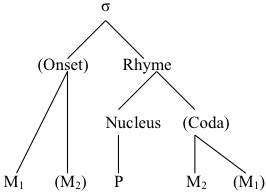
\includegraphics[scale=.45]{../figures/montano_SMAsyllable.jpg} %in the [] brackets you will determine the dimensions of your figure you will use width=3cm, height=4cm, scale=.5, angle=45 % you will play with these until the image displays correctly
    \caption{Syllable structure in the Split Margin Approach (\textit{ibid.})}
    \label{fig:montano:SMAsyllable}
\end{figure}

\noindent Syllable-internal structure in the \textsc{sma} encodes the cross-linguistic tendency for low sonority segments to occupy an M\textsubscript{1} position (a singleton onset, the first segment of an onset cluster or the second segment of a coda cluster) and for high sonority segments to occupy an M\textsubscript{2} position (the second segment of an onset cluster, a singleton coda, or the first segment of a coda cluster), as formalized in two universal relative markedness hierarchies governing M\textsubscript{1} and M\textsubscript{2} segments:
\ea \label{ex:montano:4} 
\ea Relative markedness hierarchy for M\textsubscript{1} segments (\textit{ibid.}):\\
	*M\textsubscript{1}/[r] » *M\textsubscript{1}/[l] » *M\textsubscript{1}/Nas » *M\textsubscript{1}/S » *M\textsubscript{1}/Obs\textsubscript{[+voice]} » *M\textsubscript{1}/Obs\textsubscript{[-voice]}\\
\ex Relative markedness hierarchy for M\textsubscript{2} segments (\textit{ibid.}):\\
		*M\textsubscript{2}/Obs\textsubscript{[-voice]} » *M\textsubscript{2}/Obs\textsubscript{[+voice]} » *M\textsubscript{2}/S » *M\textsubscript{2}/Nas » *M\textsubscript{2}/[l] » *M\textsubscript{2}/[r]\\
\z\z
\noindent In (\ref{ex:montano:4}), I make two adjustments to Baertsch and Davis' M\textsubscript{1} and M\textsubscript{2} hierarchies, as has been justified previously for the \textsc{sma} on a language-specific basis \citep{BaertschDavis2009}.  First, I include the sonority class of sibilants, which show greater sonority than other obstruents in OF given their inability to form obstruent-liquid onset clusters and their survival as codas beyond the GR period \citep{Pope1952, Gess1999}.  I also separate out voiced obstruents from lower sonority voiceless obstruents, as has been previously justified for sonority-sensitive markedness constraints on a language-specific basis (cf. \citet{Gouskova2004, PonsMoll2011}; see \citet{GreenBaertsch2014} for an application of the \textsc{sma} in Bamana).

Local conjunction of the M\textsubscript{1} and M\textsubscript{2} hierarchies within the syllable and word domains yields constraints on syllable-internal clusters — onset clusters (M\textsubscript{1}M\textsubscript{2}]\textsubscript{σ}) or coda clusters (M\textsubscript{2}M\textsubscript{1}]\textsubscript{σ}) — and clusters spanning across syllables but within the word, i.e. \textsc{scc}s: M\textsubscript{2}.M\textsubscript{1}]\textsubscript{ω}.  The hierarchy of conjoined split-margin constraints in the syllable domain is presented below in \figref{fig:montano:SMAsyllablehierarchy}:

\begin{figure}
    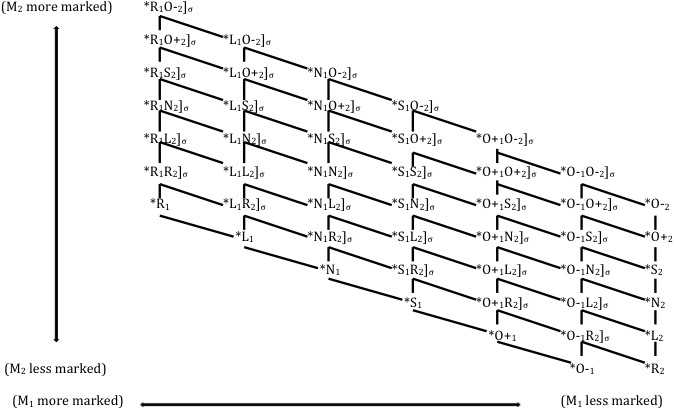
\includegraphics[scale=.5]{../figures/montano_SMAsyllablehierarchy.jpg} %in the [] brackets you will determine the dimensions of your figure you will use width=3cm, height=4cm, scale=.5, angle=45 % you will play with these until the image displays correctly
    \caption{Conjoined split-margin constraint hierarchy, syllable domain\\ *Shorthand for \textsc{sma} constraints: O = Obs; O± = Obs\textsubscript{[±voice]}; ]\textsubscript{σ} = syllable domain; ]\textsubscript{ω} = word domain; *S\textsubscript{1} = *M\textsubscript{1}/S; *S\textsubscript{1}O\textsubscript{2} =  *M\textsubscript{1}/S\&M\textsubscript{2}/Obs}
    \label{fig:montano:SMAsyllablehierarchy}
\end{figure}

\noindent The word-level hierarchy is nearly identical but is instead indexed for the word domain (\textsubscript{ω}) and must be read backwards for \textsc{scc}s: Y\textsubscript{2}.X\textsubscript{1}]\textsubscript{ω} violates *X\textsubscript{1}Y\textsubscript{2}]\textsubscript{ω}.  Since violating the syllable-level constraint necessarily entails violating the same word-level constraint, the \textsc{sma} predicts that the former will universally dominate the latter, thereby capturing the cross-linguistic tendency for a language's onset clusters (M\textsubscript{1}M\textsubscript{2}]\textsubscript{σ}) to form a subset of its possible mirror-image \textsc{scc}s (M\textsubscript{2}.M\textsubscript{1}]\textsubscript{ω}).

Applied to the intersection of prothesis and coda /s/ deletion, the universal ranking of conjoined split-margin constraints accurately predicts the four and only four attested stages of [s] realization in /sC/ clusters from Latin through OF, as well as the chronology of these stages, constituting compelling evidence for its relevance in capturing the evolution of both syllable-initial S\textsubscript{1}O\textsubscript{2} clusters and S\textsubscript{2}.O\textsubscript{1} \textsc{scc}s in GR.  These stages are presented below in \tabref{tab:1:SMApredictions}:

\begin{table}
\caption{\textsc{sma} predictions on [s]-clusters from Latin through OF}
\label{tab:1:SMApredictions}
\begin{tabular}{llll}
\lsptoprule
& Constraint ranking&	\multicolumn{2}{l}{Surface [s]-clusters}\\
\midrule
Latin & FAITH, *S\textsubscript{1}O-\textsubscript{2}]\textsubscript{σ} (» *S\textsubscript{1}O-\textsubscript{2}]\textsubscript{ω}) »&[s-Obs] onsets: & \langscicheckmark\\ 
 & \indent *O+\textsubscript{1}S\textsubscript{2}]\textsubscript{ω} » *O-\textsubscript{1}S\textsubscript{2}]\textsubscript{ω}	& [s-Obs\textsubscript{+}] \textsc{scc}s: & \langscicheckmark\\
 & & [s-Obs\textsubscript{-}] \textsc{scc}s: & \langscicheckmark\\
\midrule
Late Lat.& *S\textsubscript{1}O-\textsubscript{2}]\textsubscript{σ} » FAITH (» *S\textsubscript{1}O-\textsubscript{2}]]\textsubscript{ω}) »&[s-Obs] onsets: & \ding{55}\\
thru& *O+\textsubscript{1}S\textsubscript{2}]\textsubscript{ω} » *O-\textsubscript{1}S\textsubscript{2}]\textsubscript{ω} &[s-Obs\textsubscript{+}] \textsc{scc}s: & \langscicheckmark\\
early OF & &[s-Obs\textsubscript{-}] \textsc{scc}s: & \langscicheckmark\\
\midrule
Mid-OF & *S\textsubscript{1}O-\textsubscript{2}]\textsubscript{σ} (» *S\textsubscript{1}O-\textsubscript{2}]\textsubscript{ω}) » *O+\textsubscript{1}S\textsubscript{2}]\textsubscript{ω} »& [s-Obs] onsets: & \ding{55}\\
 & FAITH » *O-\textsubscript{1}S\textsubscript{2}]\textsubscript{ω} & [s-Obs\textsubscript{+}] \textsc{scc}s: & \ding{55}\\	
 & & [s-Obs\textsubscript{-}] \textsc{scc}s: & \langscicheckmark\\
\midrule
Late OF & *S\textsubscript{1}O-\textsubscript{2}]\textsubscript{σ} (» *S\textsubscript{1}O-\textsubscript{2}]\textsubscript{ω}) » *O+\textsubscript{1}S\textsubscript{2}]\textsubscript{ω} »& [s-Obs] onsets: & \ding{55}\\
& *O-\textsubscript{1}S\textsubscript{2}]\textsubscript{ω} » FAITH & [s-Obs\textsubscript{+}] \textsc{scc}s: & \ding{55}\\
&  & [s-Obs\textsubscript{-}] \textsc{scc}s: & \ding{55}\\
\lspbottomrule
\end{tabular}
\end{table}

\noindent The present analysis will concern itself with diachronic periods \ref{ex:montano:3ab} (pre-coda /s/ deletion), \ref{ex:montano:3ac} (Stage 1 coda /s/ deletion), and \ref{ex:montano:3ad} (Stage 2 coda /s/ deletion) above.

The catch-all FAITH constraint cited in \tabref{tab:1:SMApredictions} for expository reasons must be dismantled to properly illustrate how prothesis and /s/-deletion function in tandem to satisfy markedness constraints. Coda /s/ deletion entails a violation of a \textsc{max}(-C) constraint (no consonant deletion) to satisfy the split-margin constraint banning \textsc{scc}s with an excessively shallow fall in sonority (*X\textsubscript{1}S\textsubscript{2}]\textsubscript{ω}).  Prothesis, on the other hand, violates a \textsc{dep} constraint (no segmental insertion) to fulfill the conditions of high-ranking *\textsc{adjunct} (no adjoining a segment to the syllable node \citep{Barlow2001}), presumably lower-ranked in Latin when /s/-adjuncts were permitted, and *S\textsubscript{1}O-\textsubscript{2}]\textsubscript{σ} (no sibilant-obstruent clusters in the syllable).

It is relevant that OF vowel insertion occurs only at word margins — for example, to resyllabify prothesis clusters — and not word-medially.  Medial vowel epenthesis is unattested to my knowledge in OF, as it would run counter to constraints conspiring against pre- and post-tonic medial vowels in open syllables, deleted diachronically in an ongoing syncope process from Late Latin through GR.  The prosodic patterns established by syncope were either still phonologically imposed or retrievable in OF, as syncope applies even in loanwords from Latin fitting its requirements (cf. 12th c. loanwords \textit{ordine} > \textit{ordre}, \textit{titulu} > \textit{titre} \citep{Pope1952}).  Given this evidence, as well as the diachronic reality that prothesis had applied throughout early French long before the onset of coda /s/ deletion, context-free \textsc{dep}-V (no insertion of a vowel) must rank below an O(UTPUT)-CONTIGUITY-V constraint (no insertion within a contiguous segmental string \citep{Krämer2005}).  O-CONTIGUITY-V differs from \textsc{dep}-V in that the former bars medial epenthetic vowels interrupting the input string but not those inserted at the margins, since the sequential integrity of the underlying string is respected.

Since prothesis of word-initial /sC/ clusters is preferred over word-initial /s/-deletion, \textsc{max} must outrank \textsc{dep-v}, allowing insertion, but rank below O-CON-TIGUITY-V, since word-medially deletion is more harmonic than insertion.  I incorporate this ranking into the OF constraint hierarchies below:

\ea \label{ex:montano:5} OF constraint hierarchies for three stages of coda /s/ deletion\\
\ea\label{ex:montano:5a} early OF: before coda /s/ deletion, including word-level prothesis\\
% \scriptsize{*\textsc{Adjunct}, *S\textsubscript{1}O\textsubscript{+2}]$_\sigma$ » *S\textsubscript{1}O\textsubscript{-2}]$_\sigma$ » O-\textsc{Contiguity}-V » \textsc{Max} » \textsc{Dep-V} » *O\textsubscript{+1}S\textsubscript{2}]$_\omega$ » *O\textsubscript{-1}S\textsubscript{2}]$_\omega$}\\
%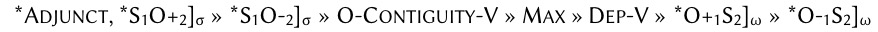
\includegraphics[scale=.375]{../figures/montano_OFranking1.jpg}

% tikzpicture for consistency with examples b and c
\begin{tikzpicture}
\footnotesize
\node[draw=none,fill=none, text height=.7em] (1) {*\textsc{Adjunct}, *S\textsubscript{1}O\textsubscript{+2}]$_\sigma$ » *S\textsubscript{1}O\textsubscript{-2}]$_\sigma$ » O-\textsc{Contiguity}-V » \textsc{Max} » \textsc{Dep-V} » *O\textsubscript{+1}S\textsubscript{2}]$_\omega$ » *O\textsubscript{-1}S\textsubscript{2}]$_\omega$};
%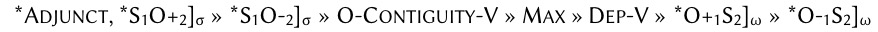
\includegraphics[scale=.375]{../figures/montano_OFranking1.jpg};
\end{tikzpicture}

\ex\label{ex:montano:5b} ca. 12th c.: Stage 1 coda /s/ deletion before voiced obstruents\\
%%% Without arrow:
% \scriptsize{*\textsc{Adjunct}, *S\textsubscript{1}O\textsubscript{+2}]$_\sigma$ » *S\textsubscript{1}O\textsubscript{-2}]$_\sigma$ » *O\textsubscript{+1}S\textsubscript{2}]$_\omega$ » O-\textsc{Contiguity}-V » \textsc{Max} » \textsc{Dep-V} » *O\textsubscript{-1}S\textsubscript{2}]$_\omega$}\\

%%% With arrow:
\begin{tikzpicture}
\footnotesize
\node[draw=none,fill=none, text height=.7em] (1) {*\textsc{Adjunct}, *S\textsubscript{1}O\textsubscript{+2}]$_\sigma$ » *S\textsubscript{1}O\textsubscript{-2}]$_\sigma$ »};
\node[draw=none,fill=none, text height=.7em] (2) [right=2cm of 1]{*O\textsubscript{+1}S\textsubscript{2}]$_\omega$};
\node[draw=none,fill=none, text height=.7em] (3) [right=-.1cm of 2]{» O-\textsc{Contiguity}-V » \textsc{Max} » \textsc{Dep-V}};
\node[draw=none,fill=none, text height=.7em] (4) [right=-.1cm of 3]{»};
\node[draw=none,fill=none, text height=.7em] (5) [right=-.2cm of 4]{*O\textsubscript{-1}S\textsubscript{2}]$_\omega$};
\draw[-Latex] (4.south) -- +(0,-0.3)-| node[below right]{} (2);
\end{tikzpicture}

%%% Original image:
% 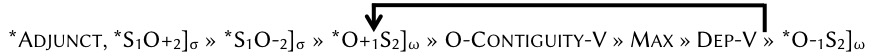
\includegraphics[scale=.375]{../figures/montano_OFranking2.jpg}

\ex\label{ex:montano:5c} ca. 13th c. : Stage 2 coda /s/ deletion before voiceless obstruents\\
%%% Without arrow:
% \scriptsize{*\textsc{Adjunct}, *S\textsubscript{1}O\textsubscript{+2}]$_\sigma$ » *S\textsubscript{1}O\textsubscript{-2}]$_\sigma$ » *O\textsubscript{+1}S\textsubscript{2}]$_\omega$ » *O\textsubscript{-1}S\textsubscript{2}]$_\omega$ » O-\textsc{Contiguity}-V » \textsc{Max} » \textsc{Dep-V} »}\\

%%% With arrow:
\begin{tikzpicture}
\footnotesize{
\node[draw=none,fill=none, text height=.7em] (1) {*\textsc{Adjunct}, *S\textsubscript{1}O\textsubscript{+2}]$_\sigma$ » *S\textsubscript{1}O\textsubscript{-2}]$_\sigma$ » *O\textsubscript{+1}S\textsubscript{2}]$_\omega$ »};
\node[draw=none,fill=none, text height=.7em] (2) [right=-.6cm of 2]{*O\textsubscript{-1}S\textsubscript{2}]$_\omega$};
\node[draw=none,fill=none, text height=.7em] (3) [right=-.1cm of 2]{» O-\textsc{Contiguity}-V » \textsc{Max} » \textsc{Dep-V}};
\node[draw=none,fill=none, text height=.7em] (4) [right=-.1cm of 3]{»};
}
\draw[-Latex] (4.south) -- +(0,-0.3)-| node[below right]{} (2);
\end{tikzpicture}

%%% Original image:
% 
\includegraphics[scale=.375]{../figures/montano_OFranking3.jpg}\\
\z\z

\noindent Subject to these constraint hierarchies, underlying word-initial /sC/ faces a new and insurmountable markedness hurdle to output realization once coda /s/ deletion becomes active (\ref{ex:montano:5b}--\ref{ex:montano:5c}). Initial /s/ essentially has nowhere to go without incurring a fatal violation: it cannot surface as an adjunct (*\textsc{adjunct}), nor in an onset cluster (*S\textsubscript{1}O-\textsubscript{2}]\textsubscript{σ}), nor as the M\textsubscript{2} of a \textsc{scc} resulting from prothesis (*X\textsubscript{1}S\textsubscript{2}]\textsubscript{ω}).  Simple vowel insertion via prothesis is thus no longer an option as in previous diachronic periods.  At this point, \textsc{max} becomes the minimal violation in both prothesis clusters and word-medially, and /s/ must delete.  But we know that this is not the whole story: though /s/ deletes in prothesis clusters, the prothetic vowel is still generated by the phonology in the input-output mapping /sC.../ $\rightarrow$ [eC...] in a curious example of not-surface-apparent opacity \citep{McCarthy1999}.

But what exactly motivates word-initial [e] once the /s/ of prothesis clusters is gone?  The crucial detail lies in the compensatory lengthening effect of coda /s/ deletion.  What ties the opaque /sC/ $\rightarrow$ [eC] mapping and the long vowel outcome of coda /s/ deletion (/VS/ $\rightarrow$ [VV]) is the \textit{surfacing of a non-underlying vocalic element}.  I argued above that a moraic account does not provide a convincing analysis on several grounds.  But if not mora preservation, then what motivates word-medial compensatory lengthening?  I claim it is the segment's root node itself, which, as part of the input phonological structure, can conceivably be preserved either by its association to an adjacent segment (compensatory lengthening) or segmental insertion (akin but not phenomenologically equivalent to prothesis).

Cross-linguistically but especially for French, the explanatory value and the phonological reality of underlying skeletal or syllabic structure have provided convincing analyses of abstract phenomena in French, such as phonologized empty onsets or skeletal slots for \textit{h aspiré} behavior \citep{Durand1986} and lexically-marked onset or nuclear word-initial glides \citep{KayeLowenstamm1984}.  Earlier in French diachrony, GR obstruent gemination in O\textsubscript{1}O\textsubscript{2} \textsc{scc}s (e.g. Lat. \textit{rupta} > GR \textit{rotta}, etc. \citep{Pope1952, Gess2004}) likely stems from faithfulness demands to preserve skeletal or root structure despite markedness.  \citet{FaustScheer2018} argue that pertinent syllabification information may be encoded during lexicalization and constitute underlying phonological material.  Therefore, I propose a high-ranking \textsc{max}(\textsc{root}) constraint requiring a root node in the input be associated with a segment (not necessarily the underlying one) in output.

This is not incompatible with Gess' (\citeyear{Gess1998, Gess1999}) astute observation that sub-segmental features compatible with vocalic realization, like [nasal] or [back], were preserved despite segment deletion in other OF coda phenomena like nasal stop deletion and /l/ vocalization.  As /s/ (or its lenited allophone before it deleted, [h] \citep{Pope1952, Gess1999}], a laryngeal lacking place features) presumably does not possess articulatory features compatible with vocalic realization, the preserved root node associates to the preceding vocalic element upon /s/ deletion, without any featural carry-over, yielding a lengthened vowel, as in (\ref{ex:montano:6}):

\ea \label{ex:montano:6} Effect of \textsc{max}(\textsc{root}): vowel lengthening with medial /s/ deletion
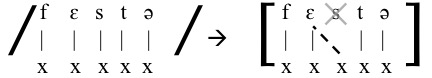
\includegraphics[scale=.4]{../figures/montano_MAXRootMedial.jpg}
\z
\noindent In prothesis clusters, though initial /s/ must delete, \textsc{max}(\textsc{root}) enforces the preservation of its root node.  With no eligible neighboring segment, this is only achievable by the insertion of some harmonic segment to overtake and license the root node.  The only segment that can possibly precede the obstruent due to split-margin constraints (*[mp...]σ, *[lp...]σ, *[rp...]σ, etc.) is a vowel, and so [e] – likely a word-initial variant of [ə], the least marked vowel in OF – fills the position.  The segmental replacement of /s/ in prothesis clusters is shown in (\ref{ex:montano:7}):
\ea \label{ex:montano:7} Effect of \textsc{max}(\textsc{root}): segment replacement in prothesis clusters

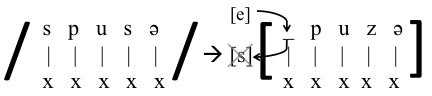
\includegraphics[scale=.4]{../figures/montano_MaxRootProthesis.jpg}
\z
\noindent With only one root node to fill, the epenthetic vowel is short.  If this analysis is correct, then prothesis in later OF is no longer vowel insertion before an illicit word-initial cluster; rather, it has transformed into outright segment replacement.

The present analysis does not crucially hinge on the claim that the epenthetic vowel is a word-initial variant of [ə], but I believe there is convincing support for this.  As others have observed \citep{Anderson1982, dell1995}, schwa is never word-initial in standard Hexagonal French, nor in OF, to my knowledge, either.  Schwa, in early as well as Modern French, always appears after an onset consonant in mono- and polysyllables, cannot solely constitute a word as other vowels can (\textit{ou} [u], \textit{à} [a], \textit{eau} [o], \textit{eu} [y], etc.), and demonstrates vowel quality alternations (to [ɛ], [ø], [œ]) when tonic \citep{Anderson1982, dell1995} or in the metrically strong position of a foot \citep{Montreuil2002}.  As \citet{Montreuil2002} claims, in the weak position of a foot, like word-finally, schwa surfaces as zero (∅).  Although in GR and OF a true phonetic [ə] \citep{Pope1952, Montreuil2002} is the correlate of the Modern French [∅] alternant of schwa, it patterns similarly in two ways.  First, in prosodically prominent positions it alternates in vowel quality with [e/ɛ] (e.g. \textit{ap}[ə]\textit{ler} 'call-\textsc{inf}' \~{} \textit{ap}[e>ɛ]\textit{le} 'call-3SG' \citep{Pope1952, Rainsford2020}), and second, as a centralized vowel \citep{Pope1952}, OF schwa likely lacked place features as Modern French schwa does in its empty nucleus characterization \citep{Anderson1982, Eychenne2006}.  But without a preceding onset to license it in the prothesis environment (the /s/ is not a candidate given CONTIGUITY), a lone word-initial [ə] likely constitutes an ill-formed syllable because it contains no featural information, as suggested by \citet{Rainsford2020}.  Given the requirement that this syllable be realized despite its lack of featural content in order to satisfy \textsc{max}-\textsc{root}, the featurally-defined [e] allophone of schwa is inserted instead.
	
	Under the less abstract analysis opposing mine in which the prothetic vowel became underlying before the time of coda /s/ deletion, one might surmise that if the prothetic vowel was indeed a schwa, perhaps the reason for the lack of lengthening is that schwa cannot be long (again, given its lack of place or other featural content \citep{Eychenne2006, Rainsford2020}).  While I agree that the phonological characteristics of schwa should prohibit it from being long, I find it unlikely, given no surface alternations in vowel quality in the prothesis environment, that underlying /ə/ would be posited by learners instead of /e/ or /ɛ/ once the prothetic vowel became fixed.  I would not expect underlying /ə/ to be learnable in this position, given it would always have surfaced as [ɛs.C...] in an initial closed syllable and given, to my knowledge, no other syllable-initial schwas elsewhere in the language.  So while on the one hand such an analysis may seem less abstract in that the prothetic vowel becomes underlying, positing this vowel specifically as an underlying /ə/ is very abstract.  Without alternations leading the acquirer to posit /ə/ in this position, underlying /e/ or /ɛ/ would likely be acquired instead, and thus vowel lengthening should occur upon /s/ deletion.  Since this is not the case, I leave the further consideration of a non-lengthening underlying /ə/ aside.
	
	Returning to my analysis, I present representative tableaux in (\ref{ex:montano:8}--\ref{ex:montano:10}) for \textit{hisde} 'horror,' \textit{feste} 'feast,' and \textit{espouse} 'wife' during the three diachronic constraint rankings in (\ref{ex:montano:5a}--\ref{ex:montano:5c}) with the addition of high-ranking \textsc{max}(\textsc{root}), thus illustrating the intersection of prothesis and /s/ deletion in one unified account:
	
\begin{figure}
\caption{Earlier OF prothesis with no coda /s/ deletion: ranking in (\ref{ex:montano:5a})} 
\label{ex:montano:8}
\subfigure[{/isdə/ $\rightarrow$ [iz.də]}]{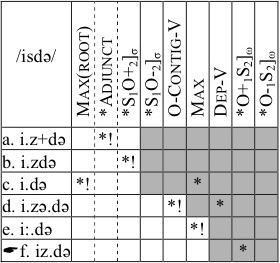
\includegraphics[height=.2\textheight]{../figures/montano_First3Tableaux1.jpg}}
\subfigure[{/fɛstə/ $\rightarrow$ [fɛs.tə]}]{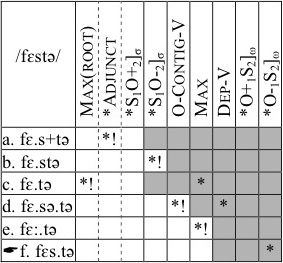
\includegraphics[height=.2\textheight]{../figures/montano_First3Tableaux2.jpg}}
\subfigure[{/spusə/ $\rightarrow$ [es.pu.zə]}]{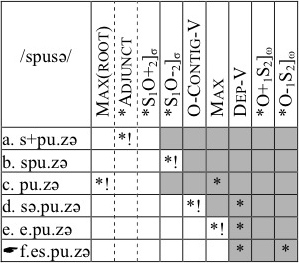
\includegraphics[height=.2\textheight]{../figures/montano_First3Tableaux3.jpg}}
\end{figure}

\begin{figure}
\caption{ca. 12th-c. OF prothesis with coda /s/ deletion, Stage 1: ranking in (\ref{ex:montano:5b})}  
\label{ex:montano:9}
\subfigure[{isdə/ $\rightarrow$ [i:.də]}]{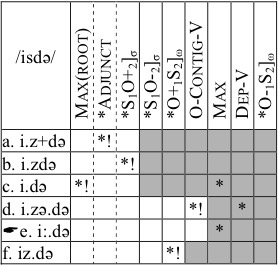
\includegraphics[height=.2\textheight]{../figures/montano_Second3Tableaux1.jpg}}
\subfigure[{/fɛstə/ $\rightarrow$ [fɛs.tə]}]{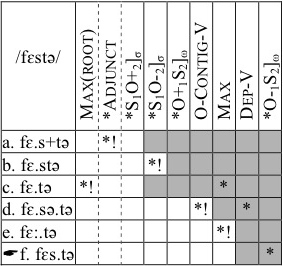
\includegraphics[height=.2\textheight]{../figures/montano_Second3Tableaux2.jpg}}
\subfigure[{/spusə/ $\rightarrow$ [es.pu.zə]}]{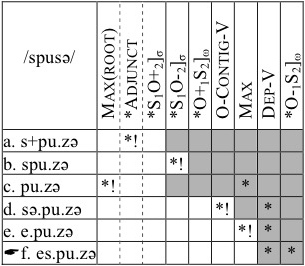
\includegraphics[height=.2\textheight]{../figures/montano_Second3Tableaux3.jpg}}
\end{figure}

\begin{figure}
\caption{ca. 13th-c. OF prothesis with /s/ deletion and coda /s/ deletion, Stage 2: ranking in
(\ref{ex:montano:5c})}  
\label{ex:montano:10}
\subfigure[{/isdə/ $\rightarrow$ [i:.də]}]{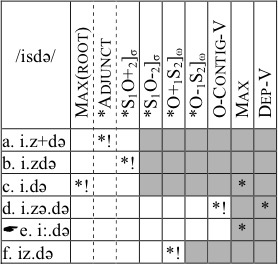
\includegraphics[height=.2\textheight]{../figures/montano_Third3Tableaux1.jpg}}
\subfigure[{/fɛstə/ $\rightarrow$ [fɛ:.tə]}]{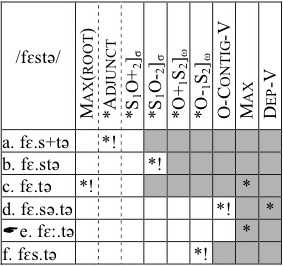
\includegraphics[height=.2\textheight]{../figures/montano_Third3Tableaux2.jpg}}
\subfigure[{/spusə/ $\rightarrow$ [es.pu.zə]}]{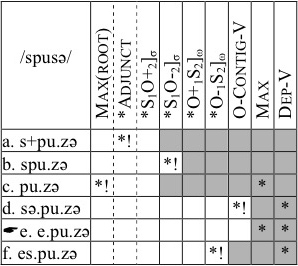
\includegraphics[height=.2\textheight]{../figures/montano_Third3Tableaux3.jpg}}
\end{figure}

\noindent As shown in (\ref{ex:montano:8}--\ref{ex:montano:10}), the constraint rankings in (\ref{ex:montano:5a}--\ref{ex:montano:5c}) not only succeed in yielding the attested output of coda /s/ deletion and prothesis during the three diachronic stages of OF, but importantly, they also illustrate how the mechanics of coda /s/ deletion overtake and fundamentally alter prothesis as a phonological process.  What superficially appears to be the application of coda /s/ deletion to prothesis clusters is in fact a different phenomenon altogether.  Since the /s/ in prothesis clusters can neither occupy the adjunct, onset, nor coda position, but its root node must be preserved, the root node of /s/ is instead filled with the only segment type, a vowel, that satisfies the markedness constraints to which it is subject.   

\section{Implications for future research and conclusions}
The analysis above succeeds in capturing the synchronic reality and phonological reflexes of both /sC/-related diachronic changes, predicated on the more abstract underlying representation of word-initial /sC/ clusters as not including the prothetic vowel.  As prothesis shifted from applying at the phrase-level phonology to the word-level no later than the 12th century, the hypothesis that prothesis clusters remained as such underlyingly not only produces the correct empirical outcome but follows the anticipated life cycle of phonological processes from phrase- to word-level, with growing opacity as the process' domain narrows \citep{Bermúdez-Otero2015}.  That word-initial /sC/ is retrievable from acquisitional input even for a short time once phrase-level surface alternations cease is not implausible, given the maintenance of supporting vowels (\textit{voyelles d'appui}) of uncertain underlying status in word-final positions (\textit{arbre} 'tree', \textit{ordre} 'order') to preserve underlying consonantal material.  Once coda /s/ deletion intersects with prothesis, however, the opaque surface realization of /sC/ as [eC] ensures the eventual irretrievability of underlying /sC/ in acquisition, paving the way for the loss of prothesis soon thereafter in Middle and Renaissance French, when /sC/-initial Latin and Italian borrowings lose the prothetic vowel in most cases.
		
If the present analysis indeed follows the life cycle of phonological processes from broader to narrower domains of application, one would anticipate that prothesis clusters are /sC/-initial at the stem-level until at least around the time of the OF intersection of prothesis and coda /s/ deletion, given that the stem-level phonology's output is the input for the word-level phonology \citep{Kiparsky2015}.  At the same time, if prothesis is presumably no longer active by the Renaissance French period, prothesis as a process should pass through the stem-level phonology (phrase > word > stem > morphology/lexicon \citep{Bermúdez-Otero2015}) on its way to becoming a relic within the lexicon (as in contemporary French \textit{éC}-initial words).  This is likely the case, based on my preliminary observations of morphophonological evidence from within OF.  Allomorph selection sensitive to vowel- or consonant-initial stems, like privative prefix \textit{de-} (pre-consonantal) \~{} \textit{des-} (pre-vocalic), though likely non-allomorphic prior to coda /s/ deletion (\textit{des-}, e.g. \textit{desranger} 'pull out of rank-\textsc{inf}', \textit{desplaire} 'displease-\textsc{inf}' \textit{desagreable} 'displeasing'), provides suggestive evidence that prothesis did not at first apply at the stem-level in OF.  Pairs such as \textit{despoir} \~{} \textit{desespoir} (/de(s) + sper/) 'makes hopeless' (e.g. "\textit{Mès une chose me despoir}," 'But one thing makes me hopeless,' from 1180 \textit{Yvain et le Chevalier du Lion} \citep{Constans1918}; cf. English loanword \textit{despair}, from OF), the latter exhibiting stem-level prothesis (cf. present-day \textit{désespérer}) and the former not, imply a narrowing of prothesis' domain from the word-level (\textit{despoir} : /sC/ is non-initial, hence no prothesis: [\textit{dé} + [\textit{spoir}...]]) to stem-level ([\textit{dés} + [\textit{espér}...]], with the prevocalic allomorph selected and prothesis applying to the stem).  Later alternating pairs like 16th-17th century \textit{dépingler} \~{} \textit{désépingler} 'unpin-\textsc{inf}' and \textit{déchouer} \~{} \textit{déséchouer} 'refloat-\textsc{inf}' are doublets preserved in the lexicon, potentially reflecting diachronically distinct treatments of stem-initial /sC/, one with stem-level prothesis and the other without.  Morphophonological data in diachrony such as these provide enticing future paths for a deeper investigation of the underlying nature of word-initial /sC/ in pre-Modern French.

In this paper, I have presented an abstract analysis that captures how the mechanics of OF prothesis and coda /s/ deletion intersect in a diachronic perspective, rooted in the attested reflexes of affected words, internal evidence within GR and OF, and suggestive morphophonological changes in attested prefixed forms.  Beyond the hypothesis of a more abstract underlying form for OF prothesis clusters, this paper additionally argues for a split-margin analysis of /s/-clusters in OF, an approach that not only formalizes the sonority sensitivity of coda /s/ deletion but inherently links two phonological processes — both targeting /sC/ clusters but in distinct prosodic positions — in ways that previous analyses of /s/ deletion like mora licensing cannot.  Finally, the opacity resulting from the segmental replacement process in my account of later OF prothesis elucidates why word-level prothesis (no longer truly prothesis in the classical sense of the term) was quickly irretrievable as a phonological process during acquisition, likely a contributing factor to the lack of prothesis in Renaissance French loanwords (cf. \citet[123--126]{Sampson2010} for a discussion of other "bottom-up," i.e. phonological-systemic, roots for prothesis loss in Renaissance French).  Following the anticipated life cycle of phonological processes \citep{Bermúdez-Otero2015}, the phenomenological evolution of prothesis in OF and its closely interrelated mechanics with respect to the contemporary coda /s/ deletion phenomenon provide meaningful systemic insights into the distinct diachronic reflexes of such clusters in French. 
\printbibliography[heading=subbibliography,notkeyword=this]

%\section*{Abbreviations}
%\begin{tabularx}{.45\textwidth}{lQ}
%... & \\
%... & \\
%\end{tabularx}
%\begin{tabularx}{.45\textwidth}{lQ}
%... & \\
%... & \\
%\end{tabularx}

%\section*{Acknowledgements}
%\citet{Nordhoff2018} is useful for compiling bibliographies

\end{document}
